% 2D periodic Fourier mode -- case_2d_mode.py.
% Doubly-periodic square, T = T0 + A sin(kx) sin(ky), k = 2 pi/L.
% Alternating hot/cold lobes (a 2D checkerboard) decay in place:
%   T0 + A sin sin * exp(-alpha * 2 k^2 t).
% A smooth periodic mode stays quiescent, so it validates the operator cleanly in
% the compressible energy path -- unlike a strong-Dirichlet plate, whose hot wall
% drives a sustained near-sonic flow.
%
% Compile:  pdflatex setup_2d_mode.tex
\documentclass[border=6pt]{standalone}
\usepackage{amsmath}
\usepackage{tikz}
\usetikzlibrary{arrows.meta}

\definecolor{coldc}{RGB}{46,86,149}
\definecolor{hotc}{RGB}{171,57,52}
\definecolor{inkc}{RGB}{30,30,30}

\begin{document}
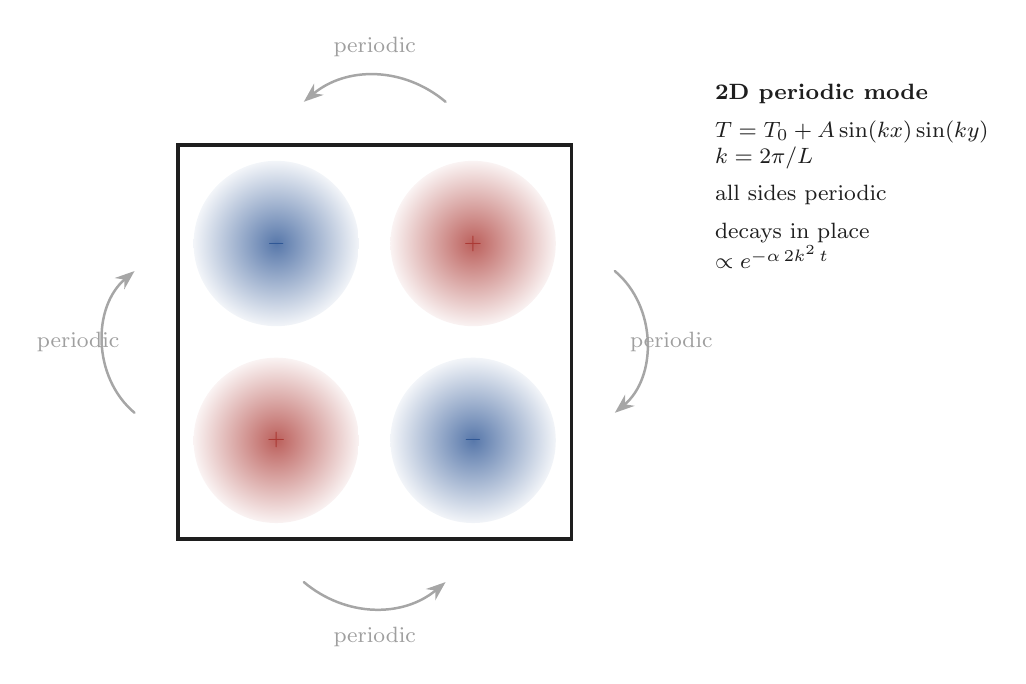
\begin{tikzpicture}[>=Stealth, font=\footnotesize, line cap=round]
  \def\S{5}

  % 2x2 checkerboard of sin*sin lobes on the square
  \foreach \i/\j/\c in {0/0/hotc, 1/0/coldc, 0/1/coldc, 1/1/hotc}{
    \shade[inner color=\c!80, outer color=\c!6]
      ({1.25+2.5*\i},{1.25+2.5*\j}) circle (1.05);
  }
  \node[hotc,  font=\footnotesize\bfseries] at (1.25,1.25) {$+$};
  \node[coldc, font=\footnotesize\bfseries] at (3.75,1.25) {$-$};
  \node[coldc, font=\footnotesize\bfseries] at (1.25,3.75) {$-$};
  \node[hotc,  font=\footnotesize\bfseries] at (3.75,3.75) {$+$};

  % square frame
  \draw[inkc, line width=1.4pt] (0,0) rectangle (\S,\S);

  % periodic-BC wrap arrows on all four sides
  \draw[->, gray!70, line width=0.9pt] (-0.55,1.6) to[out=140,in=220] (-0.55,3.4);
  \draw[->, gray!70, line width=0.9pt] (\S+0.55,3.4) to[out=-40,in=40] (\S+0.55,1.6);
  \node[gray!75, anchor=east] at (-0.62,2.5) {periodic};
  \node[gray!75, anchor=west] at (\S+0.62,2.5) {periodic};
  \draw[->, gray!70, line width=0.9pt] (1.6,-0.55) to[out=-40,in=-140] (3.4,-0.55);
  \draw[->, gray!70, line width=0.9pt] (3.4,\S+0.55) to[out=140,in=40] (1.6,\S+0.55);
  \node[gray!75, anchor=north] at (2.5,-1.0) {periodic};
  \node[gray!75, anchor=south] at (2.5,\S+1.0) {periodic};

  % annotation
  \node[inkc, anchor=west, align=left] at (\S+1.7,\S-0.4)
    {\textbf{2D periodic mode}\\[4pt]
     $T=T_0+A\sin(kx)\sin(ky)$\\
     $k=2\pi/L$\\[4pt]
     all sides periodic\\[4pt]
     decays in place\\
     $\propto e^{-\alpha\,2k^2\,t}$};
\end{tikzpicture}
\end{document}
